\subsection{A zero-shift pencil and two indexed error channels}
\label{ssec:ritz-pencil-channels}

Real-root localization through a self-adjoint quotient is already
established in Connes--van Suijlekom, Theorem~5.6 and
Proposition~5.10~\cite{CvS2025}. The following parity-squared pencil
is an explicit finite form useful for indexed error analysis; it does
not claim a new localization theorem. It separates two contributions
that a uniform convergence law must estimate.

\begin{proposition}[The arbitrary-shift virtual transform]
\label{prop:arbitrary-shift-pencil}
Use the notation of Proposition~\ref{prop:movable-symmetric-pencil}.
For a real shift $z$ with $B_z=B-zI$ invertible, define
\[
 v_z=-B_z^{-1}c,\quad q_z=B_z^{-1}w,\quad
 \sigma_z=a-z+c^Tv_z,\quad W_z=1+w^Tv_z.
\]
Let $H_z=B_z-cw^T-wc^T+(a-z)ww^T$ and
$T_z=B_zD-wr^T$. For $R_t=(D-tI)^{-1}$,
\begin{align}
 \det(T_z-tH_z)
 &=\det(B_z)\det(D-tI)\notag\\
 &\quad\cdot\{W_z[1-tw^TR_tv_z]
              -t\sigma_z w^TR_tq_z\}.
 \label{eq:arbitrary-shift-determinant}
\end{align}
If $W_z\ne0$, its roots are the movable squared-frequency roots of
the transform with central-normalized tail
$\widetilde v_z=v_z+(\sigma_z/W_z)q_z$.
\end{proposition}
\begin{proof}
Apply the two-by-two determinant lemma to
$B_z^{-1}(T_z-tH_z)$, written as $D-tI$ plus two rank-one
matrices, and use $c=D^{-1}r$ and
$[D,B]=rw^T-wr^T$. Factoring out $W_z$ gives
$1-tw^TR_t\widetilde v_z$. Polynomial continuation includes the
diagonal nodes. The movable-polynomial identity then proves the claim.
\end{proof}
The virtual transform is generally not a ground eigenstate. At the
exact ground shift $z=\varepsilon$, $\sigma_z=0$, recovering the
ground transform. At $z=0$ the pencil requires only the finite input
matrix. Its evaluation remains a spectral computation, rather than a
closed convergence formula. The arbitrary-shift determinant and
congruence identities pass 1044 exact rational checks, including
nonzero Schur complements.

\paragraph{Fixed-shift mode resolution.}
With the rectangular injection $\mathcal J=(-w,I)^T$, one has
$H_z=\mathcal J^T(A_{\rm even}-zI)\mathcal J$ and
$T_z=D^{1/2}(A_{\rm odd}-zI)D^{1/2}$.
The even trial functions vanish at the endpoints, and differentiation
maps them to the odd trial space. At fixed $C,z$, increasing $N$
therefore gives principal matrix pairs. Where the metric is positive,
min--max yields
\[
 t_k^{(N+1)}(z)\le t_k^{(N)}(z)
                  \le t_{k+1}^{(N+1)}(z).
\]
The ground shift changes with $N$, so this does not automatically
prove monotonicity for ground-transform roots. Nor does it identify
the limiting Ritz spectrum with all zeta zeros: a global space and
completeness argument are still required.
Since the movable polynomial has degree at most $N$, $N\ge k$ is
necessary to resolve a complete prefix of $k$ movable roots. It is
not sufficient; the preceding mode ladder shows substantial additional
resolution requirements. Carrier zeros cannot supply missing movable
branches.

\paragraph{Exact shift sensitivity and the minimum budget.}
For a simple branch with eigenvector $x$,
\[
 \frac{dt}{dz}
 =\frac{x^T[t(I+ww^T)-D]x}{x^TH_zx}.
\]
At a nonlattice ground root, take $x=R_tv$ and put
$\Psi(t)=1-tw^TR_tv$ and $h(t)=r^TR_tv$. Then
\[
 x^T[t(I+ww^T)-D]x=1/t-v^TR_tv,\qquad
 x^TH_\varepsilon x=h(t)\Psi'(t)/t.
\]
Equivalently, the previous divided-vector observables give
$\nu'(\varepsilon)=-S/(J(\nu)-\varepsilon\|b_\nu\|^2)$.
The full residual term is necessary for approximate states. This
endpoint derivative is not the integrated shift and is not the
displacement from a reference zero. Along a continuously matched
simple branch, the exact decomposition is
\[
 \nu_k(\varepsilon)-\gamma_k
 =\underbrace{\nu_k(0)-\gamma_k}_{\text{finite zero-shift error}}
  +\underbrace{\int_0^\varepsilon\nu_k'(z)\,dz}_{\text{energy-shift error}}.
\]
If both relative channel errors are positive and have depths $D_R,D_E$,
their total depth is exactly
\[
 D=\min(D_R,D_E)
       -\log_{10}(1+10^{-|D_R-D_E|}).
\]
For bounds on the magnitudes of the relative channel errors, adding
an arithmetic channel $10^{-D_P}$ instead gives
\[
 D_{\rm total}\ge-\log_{10}
       (10^{-D_R}+10^{-D_E}+10^{-D_P})
 \ge\min(D_R,D_E,D_P)-\log_{10}3.
\]
Thus a minimum budget has an exact error-sum basis, conditional on
quantitative channel bounds and indexed admissibility. It cannot
assign a meaningful convergence depth to an unresolved branch.
The earlier indexed residual estimate supplies a conditional
$P$-dependent arithmetic channel. Uniform $C,N,k$ estimates for
the other channels, their slopes and branch resolution remain open.

\paragraph{A certified thousand-root zero-shift prefix.}
At $C=250,N=1500$, residual-aware scalar identities certify the virtual
tail of the analytic zero-shift pencil. In particular, for point solves
$v_p,q_p$ and residuals $e=Bv_p+c$, $e_q=Bq_p-w$,
\[
 \sigma=a+c^Tv_p+v_p^Te-e^TB^{-1}e,\qquad
 W=1+w^Tv_p-q_p^Te+e_q^TB^{-1}e.
\]
The previously certified lower bound $B\succeq gI>0$ bounds the
quadratic remainders. These identities and the indexed response
identities pass 135 additional exact rational checks.
The first certificate encloses and counts all 1000 roots but cannot
resolve displacement signs at indices 1--25. Increasing only point-solve
precision leaves that limitation unchanged. The analytic assembly,
requested at 2500 decimal digits, has some interval radii of order
$10^{-2320}$; requested precision is not a certified error bound.

Reassembling the same analytic matrix at 3000 decimal digits gives
6004 refined generator enclosures contained in their earlier bounds.
The resulting norm error bound for the saved virtual coefficients is
$1.087\cdot10^{-1321}$. Interval-Newton root inclusions and an interval
polynomial Descartes upper count now certify exactly 1000 distinct
positive movable roots below $t=1555864$, one in each of the first
1000 reference windows. All 1000 displacements are strictly positive.
For indices $1,19,100,250,500,750,1000$, their relative depths are,
respectively,
\[
1180.20046,\ 1141.72691,\ 1036.95900,\ 886.65473,\
675.44086,\ 488.28489,\ 306.46160.
\]
This certifies the finite analytic zero-shift pencil, not a global
limit or every corresponding analytic ground-transform displacement.
The initial unresolved signs and all precision refinements are retained.
This limitation concerns verification widths in the independent analytic
assembly.

\paragraph{The remaining fraction depends strongly on the index.}
Comparing the saved point transforms, the ratio
$(\nu_k(0)-\gamma_k)/(\nu_k(\varepsilon)-\gamma_k)$ at
$N=1500$ rises strictly at all 999 successive steps, from
$1.57863\cdot10^{-5}$ to $0.27359962$.
At $N=500$, the fixed sparse probe gives $0.00012010$ at $k=1$
and $0.87358620$ at $k=362$.
The point comparisons therefore show that discarding the zero-shift
channel becomes increasingly inaccurate near the resolution edge.
The positive zero-shift certificate above does not silently upgrade
these two-source comparisons to analytic ground-root certificates.

A predeclared exploratory closure tests the simpler candidate
\[
 \widehat\delta_k=
 \frac{\varepsilon\nu_k'(\varepsilon)}{2A_k-1},\qquad
 A_k=\frac{F_0'(\nu_k(\varepsilon))}
               {F_\varepsilon'(\nu_k(\varepsilon))},
\]
with both transforms central-normalized. The closure is unproved;
the exact pencil derivative does not prove it. No measured reference
displacement enters its construction, and no constants are fitted.
At $N=1500$ it passes the correct-sign and $1\%$ gate for all 1000
targets, with worst relative error $0.00132420$ (about $0.13242\%$).
At $N=500$ it passes only 302/362 targets: every index 303--362 fails,
and the maximum error is $7.94672\%$. It is thus falsified as a uniform
replacement for the stronger neighbor-based predictor. The failed
closure remains useful evidence about the missing boundary response,
not a valid uniform convergence formula.

\begin{figure}[htbp]
\centering
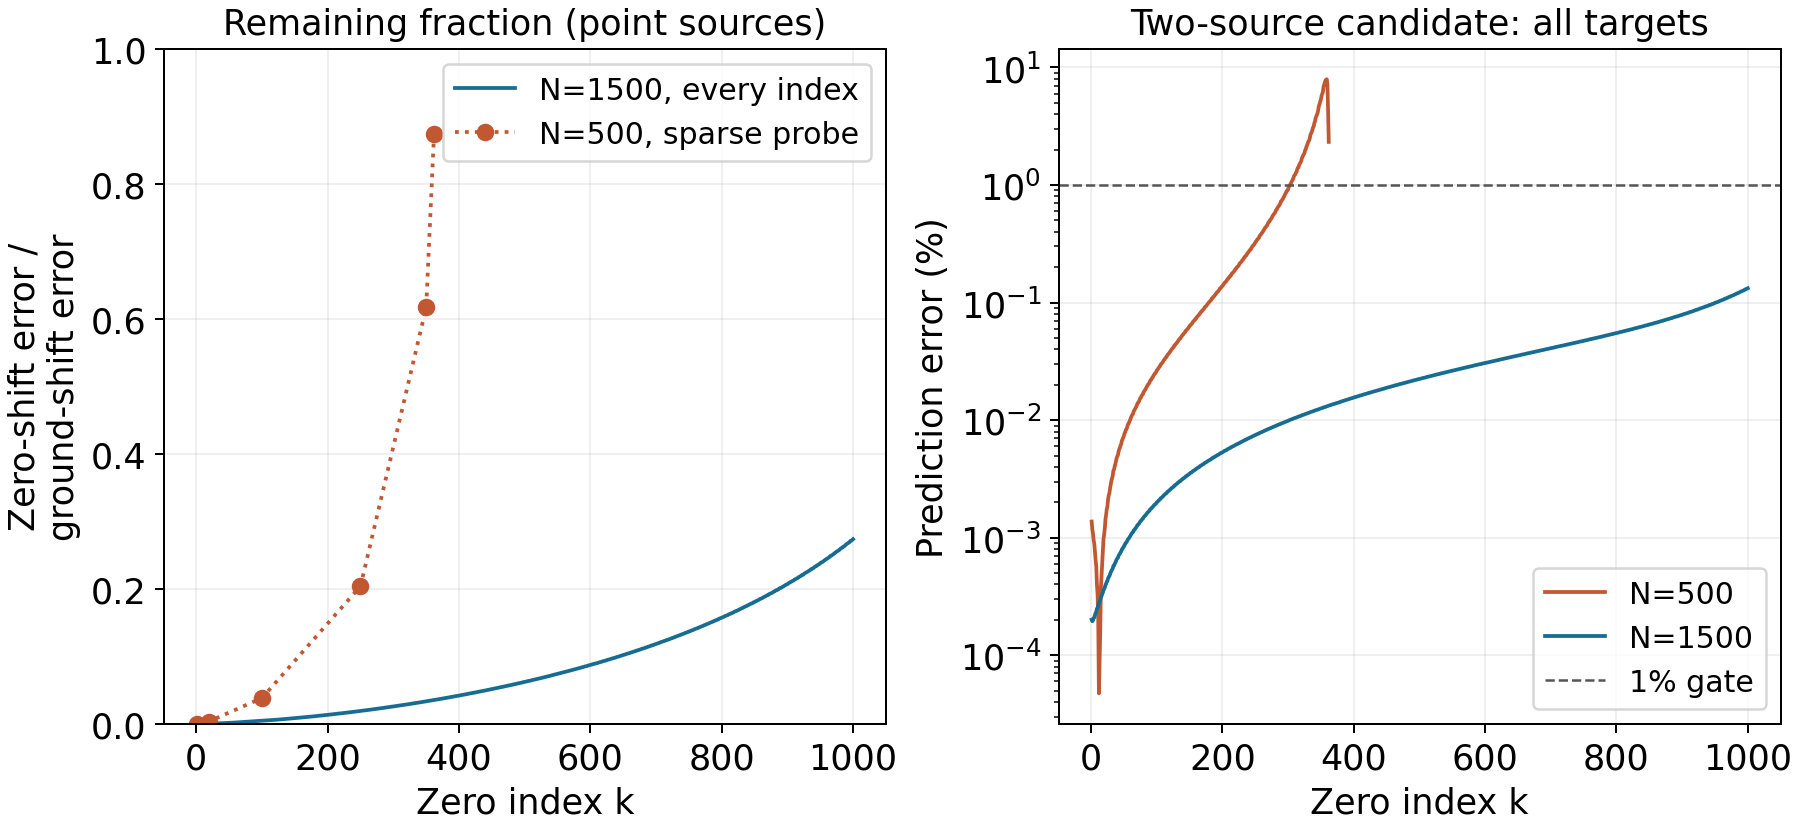
\includegraphics[width=\textwidth]{figures/ritz_pencil.png}
\caption{Two contributions and an unsuccessful simplification, at $C=250$.
Left: the remaining zero-shift fraction of the point ground error,
including the complete thousand-root comparison and the fixed sparse
lower-mode probe. Right: all targets of the unfitted two-source
candidate, including its lower-mode failures. Analytic zero-shift
root certification and point ground comparisons have distinct scopes.}
\label{fig:ritz-pencil-channels}
\end{figure}
